% Copyright (c) 2013-2017 Piotr Robert Konopelko, Core Technology Sp. z o.o.
% 
% This file is part of MooseFS.
% 
% MooseFS is free software; you can redistribute it and/or modify
% it under the terms of the GNU General Public License as published by
% the Free Software Foundation, version 2 (only).
% 
% MooseFS is distributed in the hope that it will be useful,
% but WITHOUT ANY WARRANTY; without even the implied warranty of
% MERCHANTABILITY or FITNESS FOR A PARTICULAR PURPOSE. See the
% GNU General Public License for more details.
% 
% You should have received a copy of the GNU General Public License
% along with MooseFS; if not, write to the Free Software
% Foundation, Inc., 51 Franklin St, Fifth Floor, Boston, MA 02111-1301, USA
% or visit http://www.gnu.org/licenses/gpl-2.0.html

\documentclass[a4paper,11pt,english]{report}
\usepackage{url}
\usepackage{hyperref}
\usepackage{fullpage}
\usepackage{parskip}
\usepackage{graphicx}
\usepackage{xcolor}
\usepackage{listings}

\lstset{
	language=bash,
	basicstyle=\ttfamily\scriptsize,
	showstringspaces=false,
	commentstyle=\color{black},
	keywordstyle=\color{black},
	breakatwhitespace=false,
	breaklines=true,
	showspaces=false,
	tabsize=4
}

\def\code#1{\texttt{#1}}

\newenvironment{copyrightnotice}
	{\begingroup
		\footnotesize
		\setlength{\parindent}{0pt}
		\setlength{\parskip}{\baselineskip}}
	{\endgroup}

% ------------------------------------------------------------------------

\begin{document}
	
	\renewcommand{\labelitemi}{$\bullet$}
	\renewcommand{\labelitemii}{$\circ$}
	\renewcommand{\labelitemiii}{$\bullet$}
	\renewcommand{\labelitemiv}{$\circ$}
	
	\begin{titlepage}
		\begin{center}
			
\includegraphics[width=0.2\textwidth]{images/moosefs.png}\\[1cm]
			
			% Title
			{ \huge \bfseries Installing MooseFS \\
			Step by Step Tutorial \\[0.4cm] }
			

			\textsc{Core Technology} Development \& Support Team
			
			\vfill
			
			% Bottom of the page
			{\large \today}
		\end{center}
	\end{titlepage}
	
	
	% Copyright page
	\begin{copyrightnotice}
		\begin{flushleft}
			Copyright \textcopyright{} 2013-\the\year
			\hfill
			\textsc{v. 1.5.2}\\ % DOCUMENTVERSION
			
			Piotr Robert Konopelko, \textsc{Core Technology} Development \& Support Team.
			
			\emph{Proofread by}
			Agata Kruszona-Zawadzka \\
			\emph{Coordination \& layout by} Piotr Robert Konopelko.
			
			Please send corrections to \href{mailto:peter@mfs.io}{Piotr Robert Konopelko} --  peter@mfs.io.
			
			\bigskip
			
			This file is part of MooseFS.
			
			MooseFS is free software; you can redistribute it and/or modify
			it under the terms of the GNU General Public License as published by
			the Free Software Foundation, version 2 (only).
			
			MooseFS is distributed in the hope that it will be useful,
			but WITHOUT ANY WARRANTY; without even the implied warranty of
			MERCHANTABILITY or FITNESS FOR A PARTICULAR PURPOSE. See the
			GNU General Public License for more details.
			
			You should have received a copy of the GNU General Public License
			along with MooseFS; if not, write to the Free Software
			Foundation, Inc., 51 Franklin St, Fifth Floor, Boston, MA 02111-1301, USA
			or visit \url{http://www.gnu.org/licenses/gpl-2.0.html}
		\end{flushleft}
	\end{copyrightnotice}
	
	\vfill
	
	\tableofcontents
	
	\chapter{Introduction}
	Notice: there is one dependency to resolve: users' computers need FUSE package to mount MooseFS. It can be downloaded and installed from repositories. 
	
	\section{Key differences between versions 1.6.2x and 2.0.x}
		\begin{enumerate}
			\item Master host(s) configuration is done solely via DNS -- it is no longer possible to list master(s) IP address(es) in clients' and Chunkservers' configuration; default name for master domain is \code{mfsmaster}, it can be changed in configuration files;
			\item In Pro version Metaloggers become optional, they can be replaced by additional Master Servers; in Community Edition it is still strongly recommended to set up Metaloggers.
			\item \code{Mfsmetarestore} tool is no longer present in the system; instead, it is enough to start the master process with \code{-a} switch;
			\item Configuration files now sit in \code{mfs} subdirectory inside the \code{/etc} directory (this change was introduced in 1.6.27).
		\end{enumerate}
		
		
	\section{Many Master Servers -- how does it work?}
		In previous MooseFS versions you had only one master process and any number of Metaloggers. In the event of master failure, system administrator was able to retrieve "metadata" information from the Metalogger and start a new master (on a new machine, if necessary), so the file system was up and running again. But this was always causing the system to be unavailable to clients for a period of time and required manual work to bring it back up.
	
		New MooseFS Pro version introduces many Master Servers working together in multiple roles. One role is "leader". The Leader Master is acting as it used to for the Chunkservers and clients. There is never more than one leader in any working system. 
	
		The other role is "follower". The follower master is doing what Metaloggers used to do -- it
	downloads metadata from the leader master and keeps it. But unlike a Metalogger, if a leader master stops working, a follower master is immediately ready to take on the role of leader.
	If the leader master fails, a new candidate for leader is chosen from the followers. The candidate
	assumes a role of "elect", that automatically converts to "leader" as soon as more than half of the Chunkservers connect to elect. There can be more than one follower in the system.
	
		The whole switching operation is almost invisible to the system users, as it usually takes between a couple to a dozen or so seconds. When/if the former leader master starts working again, it assumes the role of follower. If a follower master fails, it has no effect on the whole system. If such a master starts working again, it again assumes the role of follower.
		
		
	\chapter{Things to do before installation}
		For the sake of this document, it's assumed that your machines have following IP addresses:
		\begin{itemize}
			\item Master Servers: 192.168.1.1, 192.168.1.2
			\item Chunkservers: 192.168.1.101, 192.168.1.102 and 192.168.1.103
			\item Users' computers (clients): 192.168.2.x
		\end{itemize}
		
		\section{Configuring Domain Name Service}
			Before you start installing MooseFS, you need to have working DNS. It's needed for MooseFS to work properly with several Master Servers, because DNS can resolve one host name as more than one IP address.
	
			All IPs of machines, which will be Master Servers, must be included in DNS configuration file and resolved as "\code{mfsmaster}" (or any other selected name), e.g.:
	
		\begin{lstlisting}[caption={DNS entries}]
	mfsmaster	IN	A	192.168.1.1		; address of first Master Server
	mfsmaster	IN	A	192.168.1.2		; address of second Master Server
		\end{lstlisting}
		
			More information about configuring DNS server is included in a supplement to this manual.
			
		\section{Adding repository}
			To install MooseFS you need to add MooseFS Official Supported Repositories to your system. This process, both with detailed instructions for specific operating systems, is described at \url{http://get.moosefs.com} (please select your distribution in menu on the left).
			
			At this time there are repositories available for Ubuntu/Debian, RHEL/CentOS/Fedora, FreeBSD and MacOS X.
			
			\subsection{Repository branches}
				Our repository contains two branches: \code{moosefs-3} and \code{moosefs-2}. Both branches contain stable and production-ready MooseFS version.
				
				At the time of writing this guide, \code{moosefs-3} branch contains version 3.0.86-1, and \code{moosefs-2} branch contains version 2.0.91-1.
				
				\code{moosefs-3} branch is a default and you don't need to make any changes in default URL (\code{http://ppa.moosefs.com/moosefs-3/}).
				
				If you want to use \code{moosefs-2} branch, you just need to replace \code{moosefs-3} with \code{moosefs-2} after \code{http://ppa.moosefs.com/} and before \code{apt}, \code{yum}, \code{freebsd} or \code{osx}, so URL will look like:
				
				\code{http://ppa.moosefs.com/moosefs-2/[rest of url]}
				
				It is also possible to use version number instead of "branch" if you want to upgrade to a specific version of MooseFS (e.g. 3.0.81-1):
				
				\code{http://ppa.moosefs.com/3.0.81/[rest of url]}
				
				\textbf{Notice: If you want to use the last option, please remember you need to manually change version number on each server to the selected one before doing an upgrade.}
				
		\section{Differences in package names between MooseFS \\ and MooseFS Pro}
			MooseFS and MooseFS Pro packages are named according to the following pattern:
			
			\bigskip

			\begin{tabular}{l | l | l}
				\textbf{MooseFS module}	&	\textbf{MooseFS Pro}				& {\textbf{MooseFS}}			\\ \hline
				Master Server			&	\code{moosefs-pro-master}			& \code{moosefs-master}		\\ \hline
				Chunkserver				&	\code{moosefs-pro-chunkserver}	& \code{moosefs-chunkserver}	\\ \hline
				Metalogger				&	\code{moosefs-pro-metalogger}		& \code{moosefs-metalogger}	\\ \hline
				Client					&	\code{moosefs-pro-client}			& \code{moosefs-client}		\\ \hline
				CLI Interface			&	\code{moosefs-pro-cli}			& \code{moosefs-cli}			\\ \hline
				CGI Interface			&	\code{moosefs-pro-cgi}			& \code{moosefs-cgi}			\\ \hline
				CGI Server				&	\code{moosefs-pro-cgiserv}		& \code{moosefs-cgiserv}		\\ \hline
				Netdump					&	\code{moosefs-pro-netdump}		& \code{moosefs-netdump}		\\ \hline
				Supervisor				&	\code{moosefs-pro-supervisor}		& n/a
			\end{tabular}
			
			
	\chapter{MooseFS installation process on dedicated machines}
		\textbf{Notice: In this tutorial it is assumed, that you have MooseFS Community Edition. If you want to install MooseFS Pro, please use '\code{pro}' in package names, e.g.: \code{moosefs-pro-master} instead of \code{moosefs-master}.}
		
		\bigskip
		
		In this tutorial it is also assumed, that you have Ubuntu/Debian installed on your machines. If you have another distribution, please use appropriate package manager instead of \code{apt}.
		
		Notice, that most of commands below are preceded by \code{\#} sign, which means, that you have to run such command as \code{root} (\code{\$} sign means normal user). The easiest way to become \code{root} is to run:
		
		\begin{lstlisting}[caption={Becoming \code{root}}]
	$ sudo su -
		\end{lstlisting}
		
		\section{Master Server(s) installation}
			\bigskip
			
			\begin{center}
			\textbf{\fcolorbox{red}{pink}{Warning: Configuration files on all Master Servers must be consistent!}}
			\end{center}
			
			\bigskip
			\bigskip
			
			In MooseFS 2.0 Master Server (and also other modules) installation can be accomplished by running the command listed below:
			
			\begin{lstlisting}[caption={Installing Master Server}]
	# apt-get install moosefs-master
			\end{lstlisting}
			
			
			Sample configuration files will be created in \code{/etc/mfs} with the extension \code{*.sample} (MooseFS 3.0+) or \code{*.dist} (MooseFS 2.0). Use these files as your target configuration files:
			
			\begin{lstlisting}[caption={Copying default config files as target configuration files (MooseFS 3.0)}]
	# cd /etc/mfs
	# cp mfsmaster.cfg.sample mfsmaster.cfg
	# cp mfsexports.cfg.sample mfsexports.cfg
			\end{lstlisting}
			
			
			
			If you would like to change any of the settings you should uncomment the appropriate line and set a different value. For the lines which are commented the system will use built-in default values, i.e. those listed in commented lines.
			
			File \code{mfsmaster.cfg} contains Master Server settings. You can find out more information about this file in the man pages (\code{man mfsmaster.cfg} or at \url{https://moosefs.com/manpages/mfsmaster-cfg.html}).
			
			File \code{mfsexports.cfg} specifies which users' computers can mount the file system and with what
			privileges. For example, to specify that only machines addressed as \code{192.168.2.x} can use the whole structure of MooseFS resources (\code{/}) in read/write mode, in the first line which is not commented out change the asterisk (\code{*}) to \code{192.168.2.0/24}, so that you'll have:
			
			
			\begin{lstlisting}[caption={Changes to mfsexports.cfg}]
	192.168.2.0/24		/		rw,alldirs,maproot=0
			\end{lstlisting}
			
			\bigskip
			
			If you are setting up MooseFS Pro, at this point place proper \code{mfslicence.bin} file into \code{/etc/mfs} directory:
			
			\begin{lstlisting}[caption={Instaling mfslicence.bin file}]
	# cp /path/to/mfslicence.bin /etc/mfs
			\end{lstlisting}
			
			The \code{mfslicence.bin} file must be installed on all Master Servers.\\
			\code{mfslicence.bin} file is not necessary to be present on Community Edition Master Server.
			
			If you want MooseFS Master Server to start automatically during system boot, \\
			edit \code{/etc/default/moosefs-master} and set \code{MFSMASTER\_ENABLE} variable to \code{true}):
			
			\begin{lstlisting}[caption={Configuring mfsmaster autostart}]
	MFSMASTER_ENABLE=true
			\end{lstlisting}
			
			At this point it is possible to run the Master Server (using the standard way to run services):
			
			\begin{lstlisting}[caption={Starting MooseFS Master Server}]
	# service moosefs-master start
			\end{lstlisting}
			
			or:
			
			\begin{lstlisting}[caption={Starting MooseFS Master Server}]
	# mfsmaster start
			\end{lstlisting}
			
			To install second (third, etc.) Master Server just repeat steps listed above on another machine (Pro only).
			\vfill
			
		\section{MooseFS CGI and CGI Server installation}
			MooseFS CGI monitor interface is used to let user observe and analyze current MooseFS status (as you can see on screenshots presented below): \\
			
			\begin{center}
				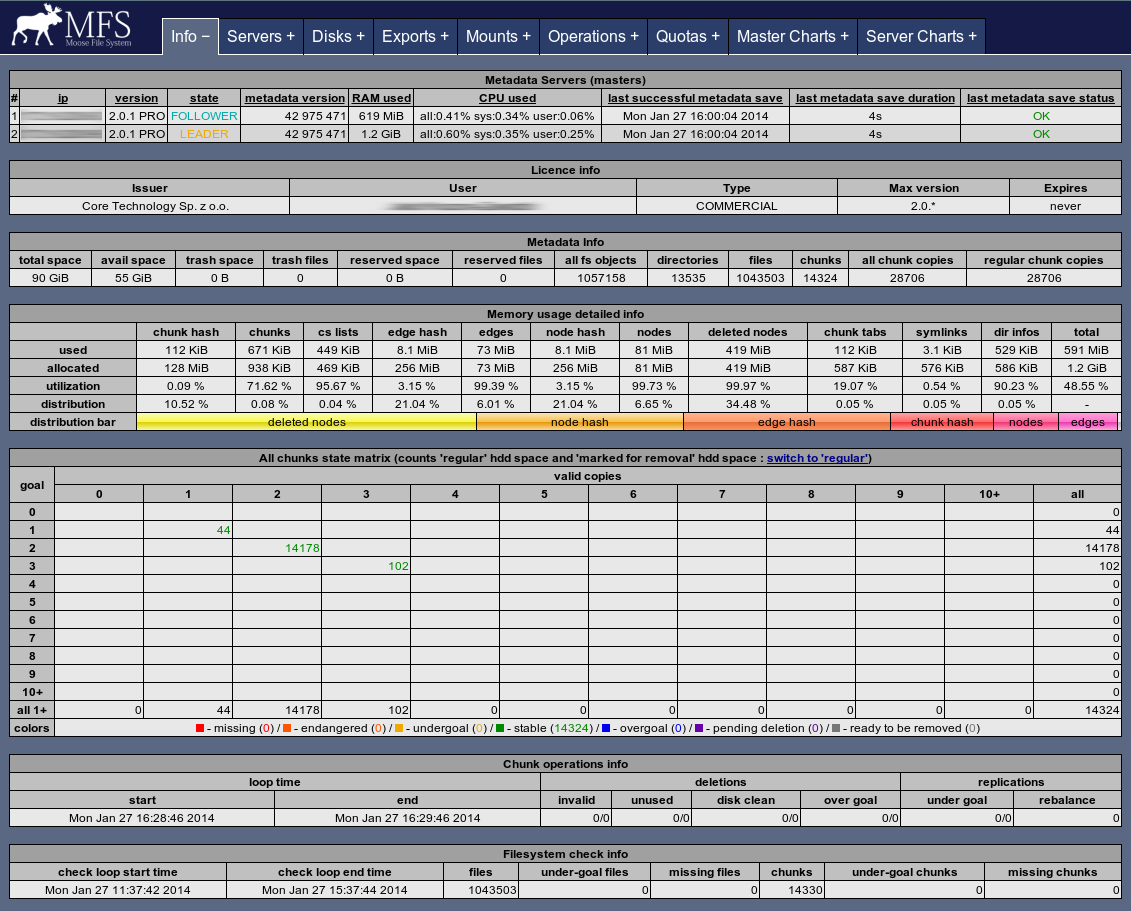
\includegraphics[width=1\textwidth]{images/mfsscr1_blur.png}\\[1cm]
				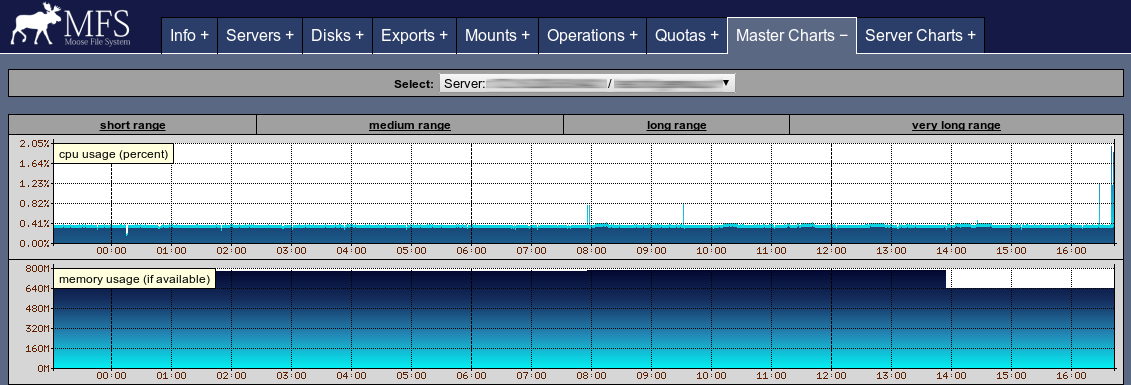
\includegraphics[width=1\textwidth]{images/mfsscr3_blur.png}\\[0.5cm]
				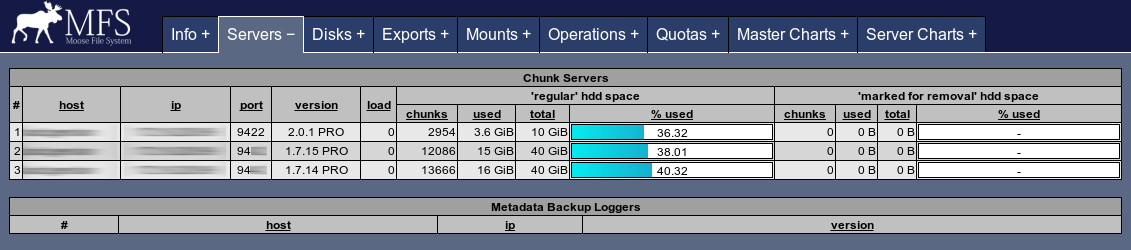
\includegraphics[width=1\textwidth]{images/mfsscr2_blur.png}\\[0.5cm]
			\end{center}
			
			\bigskip
			
			We recommend installing MooseFS CGI and CGI Server on all Master Servers.
			
			\bigskip
			
			\begin{lstlisting}[caption={MooseFS CGI and CGI Server installation}]
	# apt-get install moosefs-cgiserv
	# apt-get install moosefs-cgi
			\end{lstlisting}
			
			If you want MooseFS CGI Server to start automatically during system boot, \\
			edit \code{/etc/default/moosefs-cgiserv} and set \code{MFSCGISERV\_ENABLE} variable to \code{true}):
			
			\begin{lstlisting}[caption={Configuring mfscgiserv autostart}]
	MFSCGISERV_ENABLE=true
			\end{lstlisting}
			
			You can now run CGI Monitor Server:
			
			\begin{lstlisting}[caption={Starting MooseFS CGI Server}]
	# service moosefs-cgiserv start
			\end{lstlisting}
			
			or:
			
			\begin{lstlisting}[caption={Starting MooseFS CGI Server}]
	# mfscgiserv start
			\end{lstlisting}
			
			Information should now be available under \url{http://192.168.1.1:9425/} (for the moment there will be no data about Chunkservers).
			
			
		\section{MooseFS CLI installation}
			MooseFS Command Line Interface (CLI) tool allows you to see various information about MooseFS status. This tool has many options, which allow you to check all the information you can see in your CGI, but from command line, so it is possible to use MooseFS CLI in scripts. You can list all the options by invoking the tool with \code{-h} or \code{--help} switch or check it at \url{https://moosefs.com/manpages/mfscli.html}. E.g. \code{mfscli} with \code{-SIN} option will display basic info similar to the "Info" tab in CGI.
			
			We recommend installing MooseFS CLI on all Master Servers:
			
			\begin{lstlisting}[caption={MooseFS CLI installation}]
	# apt-get install moosefs-cli
			\end{lstlisting}
			
			
		\section{Metadata backup servers (Metaloggers) installation}
			In MooseFS Pro, when there are at least two Master Servers present, Metalogger is optional, because when leader master fails, another one takes over its work.
			
			\textbf{In MooseFS (non-Pro) we strongly recommend to set up at least one Metalogger.} \\
			
			It is recommended, that the machine used to install the backup server is as strong as the Master Server (at least in regards to the amount of RAM). In case of the Master Server failure, after importing changelogs to the
			metadata file, the Metalogger server can be easily set up to take over functions of the managing server.
			
			Issue the following commands to install and configure MooseFS Metalogger with default settings:
			
			\begin{lstlisting}[caption={Installing and configuring Metalogger}]
	# apt-get install moosefs-metalogger
		
	# cd /etc/mfs
	# cp mfsmetalogger.cfg.sample mfsmetalogger.cfg
			\end{lstlisting}
			
			For our test installation you'll leave mfsmetalogger.cfg unchanged. You can find out more information about this file in the man pages (\code{man mfsmetalogger.cfg} or at \url{https://moosefs.com/manpages/mfsmetalogger-cfg.html}).
			In case you have changed the default name \code{mfsmaster} to a different one, you need to uncomment and change the \code{MASTER\_HOST} variable in \code{mfsmetalogger.cfg} file.
			
			If you want MooseFS Metalogger to start automatically during system boot, \\
			edit \code{/etc/default/moosefs-metalogger} and set \code{MFSMETALOGGER\_ENABLE} variable to \code{true}):
			
			\begin{lstlisting}[caption={Configuring mfsmetalogger autostart}]
	MFSMETALOGGER_ENABLE=true
			\end{lstlisting}
			
			Now you are ready to start the backup server process:
			
			\begin{lstlisting}[caption={Starting MooseFS Metalogger}]
	# service moosefs-metalogger start
			\end{lstlisting}
			
			or
			
			\begin{lstlisting}[caption={Starting MooseFS Metalogger}]
	# mfsmetalogger start
			\end{lstlisting}
			
			To install second (third, etc.) Metalogger just repeat steps listed above on another machine.
			
		\section{Chunkservers installation}
			Issue the following commands on the machines which are to be Chunkservers:
			
			\begin{lstlisting}[caption={Installing MooseFS Chunkserver}]
	# apt-get install moosefs-chunkserver
			\end{lstlisting}
			
			
			Now prepare configuration files of the Chunkservers:
			
			\begin{lstlisting}[caption={Preparing configuration files}]
	# cd /etc/mfs
	# cp mfschunkserver.cfg.sample mfschunkserver.cfg
	# cp mfshdd.cfg.sample mfshdd.cfg
			\end{lstlisting}
			
			
			For our test installation you'll leave mfschunkserver.cfg unchanged. You can find out more information about this file in the man pages (\code{man mfschunkserver.cfg} or at \url{https://moosefs.com/manpages/mfschunkserver-cfg.html}).
			In case you have changed the default name \code{mfsmaster} to a different one, you also need to uncomment and change the \code{MASTER\_HOST} variable in \code{mfschunkserver.cfg} file.
			
			It is recommended that they are used exclusively for the MooseFS -- this is necessary to manage the free space properly.
			
			Let's assume, that \code{/dev/sdb} and \code{/dev/sdc} devices are designated to store chunks. First of all, create a partition table and partition on these devices. 
			\begin{lstlisting}[caption={Creating a partition on \code{/dev/sdb}}]
	# parted --align optimal /dev/sdb
	(parted) mklabel gpt
	(parted) mkpart mfschunks1 0% 100%
	(parted) q
			\end{lstlisting}
			
			\begin{lstlisting}[caption={Creating a partition on \code{/dev/sdc}}]
	# parted --align optimal /dev/sdc
	(parted) mklabel gpt
	(parted) mkpart mfschunks2 0% 100%
	(parted) q
			\end{lstlisting}
			
			Install XFS Progs:
			\begin{lstlisting}[caption={Installing \code{xfsprogs} (on Debian/Ubuntu)}]
	# apt-get install xfsprogs
			\end{lstlisting}
			
			Then, format newly created partition with XFS filesystem:
			\begin{lstlisting}[caption={Formatting partitions}]
	# mkfs.xfs /dev/sdb1
	# mkfs.xfs /dev/sdc1
			\end{lstlisting}
			
			If you have drives with 4k physical sector size (most of 2 and 4 TiB modern HDDs have 4k physical sector size), instead of the command above, issue:
			\begin{lstlisting}[caption={Formatting partitions with \code{4k} block size}]
	# mkfs.xfs -s size=4k /dev/sdb1
	# mkfs.xfs -s size=4k /dev/sdc1
			\end{lstlisting}
			
			Then, add appropriate entries into \code{/etc/fstab}:
			\begin{lstlisting}
	/dev/sdb1        /mnt/mfschunks1     xfs     defaults        0       0
	/dev/sdc1        /mnt/mfschunks2     xfs     defaults        0       0
			\end{lstlisting}
			
			Create directories for mounting newly created partitions:
			\begin{lstlisting}[caption={Creating directories}]
	# mkdir /mnt/mfschunks1
	# mkdir /mnt/mfschunks2
			\end{lstlisting}
			
			Mount newly created partitions:
			\begin{lstlisting}[caption={Mounting partitions}]
	# mount /mnt/mfschunks1
	# mount /mnt/mfschunks2
			\end{lstlisting}
			
			Change ownership and access rights to mountpoints to let MooseFS Chunkserver write to them:
			
			\begin{lstlisting}[caption={Changing ownership}]
	# chown mfs:mfs /mnt/mfschunks1
	# chown mfs:mfs /mnt/mfschunks2
	
	# chmod 770 /mnt/mfschunks1
	# chmod 770 /mnt/mfschunks2
			\end{lstlisting}
			
			At this point enter mountpoints in \code{mfshdd.cfg} file:
			\begin{lstlisting}[caption={Contents of mfshdd.cfg file}]
	/mnt/mfschunks1
	/mnt/mfschunks2
			\end{lstlisting}
			
			If you want MooseFS Chunkserver to start automatically during system boot, \\
			edit \code{/etc/default/moosefs-chunkserver} and set \code{MFSCHUNKSERVER\_ENABLE} variable to \code{true}).
			
			\begin{lstlisting}[caption={Configuring autostart of MooseFS Chunkserver}]
	MFSCHUNKSERVER_ENABLE=true
			\end{lstlisting}
			
			
			Now you are ready to start the Chunkserver:
			
			\begin{lstlisting}[caption={Starting MooseFS Chunkserver}]
	# service moosefs-chunkserver start
			\end{lstlisting}
			
			or:
			
			\begin{lstlisting}[caption={Starting MooseFS Chunkserver}]
	# mfschunkserver start
			\end{lstlisting}
			
			
			Repeat the same steps for each Chunkserver you want to use for storing data in MooseFS system.
			
			At this point, at \url{http://192.168.1.1:9425}, you should be able to see full information about the system including the Master Server and Chunkservers.
			
		\section{Users' computers installation}
			In order to mount a file system based on MooseFS, it is necessary that users' computers have FUSE package (at least in version 2.6, recommended $\geq$ 2.7.2). If it is not present, you have to install it. One of the options is to compile it from sources, or you can install it from repositories on Debian-based systems with following command:
			
			\begin{lstlisting}[caption={Installing FUSE}]
	# apt-get install fuse libfuse2
			\end{lstlisting}
			
			
			\code{mfsmount} can be installed in the same way as other MooseFS components:
			
			\begin{lstlisting}[caption={Installing mfsmount}]
	# apt-get install moosefs-client
			\end{lstlisting}
			
			Let's assume that you'll mount the system in a \code{/mnt/mfs} folder on a client's machine. Issue the following commands:
			
			\begin{lstlisting}[caption={Mounting the Moose File System}]
	# mkdir -p /mnt/mfs
	# mfsmount /mnt/mfs -H mfsmaster.host.name
			\end{lstlisting}
			
			Now after issuing the \code{df -h | grep mfs} command you should get information similar to this:
			\begin{lstlisting}[caption={Result of \code{df -h | grep mfs}}]
	/dev/sdb          2.0G    69M    1.9G    4%    /mnt/mfschunks1
	/dev/sdc          2.0G    69M    1.9G    4%    /mnt/mfschunks2
	mfsmaster:9421    3.2G    0      3.2G    0%    /mnt/mfs
			\end{lstlisting}
			
	\chapter{Basic MooseFS use}
		To create \code{folder1} in \code{/mnt/mfs}, in which you will store files in one copy (setting \code{goal=1}), issue the following command:
		
		\begin{lstlisting}[caption={Making directory \#1}]
	mkdir -p /mnt/mfs/folder1
		\end{lstlisting}
		
		To create \code{folder2}, in which you will store files in two copies (setting \code{goal=2}), issue the following command:
		\begin{lstlisting}[caption={Making directory \#2}]
	mkdir -p /mnt/mfs/folder2
		\end{lstlisting}
		
		The number of copies for the folder is set with the \code{mfssetgoal -r} command:
		
		\begin{lstlisting}[caption={\code{mfssetgoal -r command}}]
	# mfssetgoal -r 1 /mnt/mfs/folder1
	/mnt/mfs/folder1:
	inodes with goal changed:             0
	inodes with goal not changed:         1
	inodes with permission denied:        0
	
	# mfssetgoal -r 2 /mnt/mfs/folder2
	/mnt/mfs/folder2:
	inodes with goal changed:             1
	inodes with goal not changed:         0
	inodes with permission denied:        0
		\end{lstlisting}
		
		Create and copy a file to both folders:
		
		\begin{lstlisting}[caption={Creating and copying a file to newly created folders}]
	echo "test" > testmfs
	cp testmfs /mnt/mfs/folder1
	cp testmfs /mnt/mfs/folder2
		\end{lstlisting}
		
		To check in how many copies a file is stored, use the \code{mfscheckfile} command. In \code{folder1} you have one copy stored in one chunk:
		
		\begin{lstlisting}[caption={Checking amount of copies}]
	# mfscheckfile /mnt/mfs/folder1/testmfs
	/mnt/mfs/folder1/testmfs:
	chunks with 1 copy:                   1
		\end{lstlisting}
		
		And in the \code{folder2} the file \code{testmfs} is stored in two copies:
		
		\begin{lstlisting}[caption={Checking amount of copies}]
	# mfscheckfile /mnt/mfs/folder2/testmfs
	/mnt/mfs/folder2/testmfs:
	chunks with 2 copies:            1
		\end{lstlisting}
		
		Note, that if you set a goal for a file higher than the total number of working Chunkservers, this file will be saved in only as many copies as there are Chunkservers. This is because one Chunkserver will store no more than one copy of any chunk/file.
		
		You can find more information about MooseFS usage and commands on this website:
		\begin{itemize}
			\item \url{https://moosefs.com/documentation.html}
		\end{itemize}
		
		It is also recommended to read Best practices, Frequntly Asked Questions and Manpages:
		\begin{itemize}
			\item \url{https://moosefs.com/documentation/best-practices.html}
			\item \url{https://moosefs.com/documentation/faq.html}
			\item \url{https://moosefs.com/manpages.html}
		\end{itemize}
		
		
		
	\chapter{Stopping MooseFS}
		In order to safely stop the MooseFS cluster you have to perform the following steps:
		\begin{itemize}
			\item Stop all the processes which use MooseFS mounted share. \code{lsof -n | grep mfsmount} may be helpful.
			\item Unmount the file system on all machines using umount command (in our examples it would be: \code{umount /mnt/mfs})
			\item Stop the Chunkserver processes: \code{service moosefs-chunkserver stop}
			\item Stop the Master Server process(es): \code{service moosefs-master stop}
			\item Stop the Metalogger process(es) (if any): \code{service moosefs-metalogger stop}
		\end{itemize}
		
	
	\chapter{Supplement: Setting up DNS server on Debian/Ubuntu}
		
		In this extra chapter you'll use \code{bind9} as your DNS server. \\
		Notice: You can find out more about DNS server e.g. on these pages:
		
		\begin{itemize}
			\item \url{https://help.ubuntu.com/community/BIND9ServerHowto}
			\item \url{http://ubuntuforums.org/showthread.php?t=236093} \\
		\end{itemize}
		
		
		\section{Setting up DNS server}
			\begin{enumerate}
				\item The very first thing to do is installing bind9 and DNS utils. You can do this by running the following command:
					
					\begin{lstlisting}[caption={installing bind9}]
	# sudo apt-get install bind9 dnsutils
					\end{lstlisting}
					
					Main configuration files are placed in /etc/bind/ directory.
					
				\item The second thing you have to do is edit in your favorite editor (e.g. \code{nano} or \code{vim}) file named "\code{named.conf.local}". You need to add there your new zone, e.g.:
			
					\begin{lstlisting}[caption={New zone in named.conf.local}]
	zone "mfsnetwork.lan" {
	        type master;
	        file "/etc/bind/mfsnetwork.lan";
	};
					\end{lstlisting}
					
					In this file you can decide whether it is master or slave server and select path to zone's config file.
					
				\item After that create the file you've pointed to in the zone configuration (user \code{bind} must have permissions to read it) and paste there the following code:
					
					\begin{lstlisting}[caption={mfsnetwork.lan configuration file}]
	$TTL 3600
	$ORIGIN mfsnetwork.lan.
	@	IN	SOA	dns.mfsnetwork.lan.	root.mfsnetwork.lan. (
					2016032900 ; serial number YYYMMDDSS
					10800 ; refresh
					3600 ; retry
					604800 ; expire
					10800 ; negative TTL
	)
	
	@				IN	NS	dns.mfsnetwork.lan.
	@				IN	A	192.168.0.1 ; address of bind9
	dns				IN	A	192.168.0.1 ; address of bind9
	
	mfsmaster		IN	A	192.168.1.1 ; address of Master01
	mfsmaster		IN	A	192.168.1.2 ; address of Master02
	
	mfsmaster01		IN	A	192.168.1.1 ; address of Master01
	mfsmaster02		IN	A	192.168.1.2 ; address of Master02
		
	chunkserver01	IN	A	192.168.1.101 ; address of Chunkserver01
	chunkserver02	IN	A	192.168.1.102 ; address of Chunkserver02
	chunkserver03	IN	A	192.168.1.103 ; address of Chunkserver03
					\end{lstlisting}
					
				\item Next thing to do is to edit file \code{/etc/bind/named.conf.options}. You should use here your ISP's DNS servers, or you can use OpenDNS servers -- IP addresses are presented below:
					
					\begin{lstlisting}[caption={\code{named.conf.options} configuration file}]
	forwarders {
			208.67.222.222;
			208.67.220.220;
	};
					\end{lstlisting}
					
				\item Last thing to do is restarting bind9 DNS server (to let it load new configuration):
					
					\begin{lstlisting}[caption={Restarting bind9}]
	# service bind9 restart
					\end{lstlisting}
			\end{enumerate}
			
		\section{Setting up revDNS server}
			Reverse DNS server is used by MooseFS and all network services in general to translate IP addresses to human-readable form (e.g. \code{192.168.1.1} to \code{mfsmaster01}).
			Ater installing and properly configuring DNS server you need to do 3 more things to have revDNS set up:
			
			\begin{itemize}
				\item In \code{/etc/bind} directory create an empty file named \code{rev.168.192.in-addr.arpa} and paste into it the following code:
					
					\begin{lstlisting}[caption={Content of \code{rev.168.192.in-addr.arpa} file}]
	@	IN      SOA     dns.mfsnetwork.lan. root.mfsnetwork.lan. (
							2016032900 ; serial number YYYYMMDDSS
							28800
							604800
							604800
							86400
	)
	
	
	
	168.192.in-addr.arpa.	IN	NS	dns.mfsnetwork.lan.
	
	1.1						IN	PTR	mfsmaster01.mfsnetwork.lan.
	2.1						IN	PTR	mfsmaster02.mfsnetwork.lan.
	
	101.1					IN	PTR	chunkserver1.mfsnetwork.lan.
	102.1					IN	PTR	chunkserver2.mfsnetwork.lan.
	103.1					IN	PTR	chunkserver3.mfsnetwork.lan.
					\end{lstlisting}
					
				\item Add the following code to \code{/etc/bind/named.conf.local} file:
					
					\begin{lstlisting}[caption={Extra code to add to \code{/etc/bind/named.conf.local} file}]
	zone "168.192.in-addr.arpa" {
	        type master;
	        file "/etc/bind/rev.168.192.in-addr.arpa";
	};
					\end{lstlisting}
					
				\item Run \code{service bind9 restart} command:
					
					\begin{lstlisting}[caption={Running \code{service bind9 restart} command}]
	# service bind9 restart
					\end{lstlisting}
			\end{itemize}
\end{document}
